\documentclass[11pt,a4paper]{article}

\usepackage[utf8]{inputenc} 
\usepackage[T1]{fontenc} 
\usepackage{lmodern}
\usepackage[margin=2.5cm]{geometry}
\usepackage[german]{babel}
\usepackage{amsmath} 
\usepackage{graphicx} 
\usepackage{booktabs}
\usepackage{hyperref}
\hypersetup{
    colorlinks,
    citecolor=red,
    filecolor=black,
    linkcolor=black!60!blue!90!,
    urlcolor=black} 
\usepackage{nicefrac}
\usepackage[table]{xcolor}
\usepackage{tocloft}
\usepackage{wrapfig}
\usepackage{gensymb}

\setlength{\parindent}{0pt}
\setlength{\parskip}{1ex plus 0.5ex minus 0.5ex}

\definecolor{incolor}{rgb}{0.0, 0.0, 0.5}

\hbadness=99999

\newcommand{\refpy}[1]{Siehe Anhang: \textit{Rechnungen in Python} (\texttt{{\color{incolor}In [{\color{incolor}#1}]}})}
\newcommand\dif{\mathop{}\!\mathrm{d}}
\newcommand{\halftime}[4]{\begin{figure}[h]
\begin{minipage}{.#1\textwidth}#3\end{minipage}\begin{minipage}{.#2\textwidth}
\centering
#4\end{minipage}
\end{figure}}
\renewcommand{\vec}{\boldsymbol}

\begin{document}

{
\centering 
\large 
Physiklabor für Anf\"anger*innen \\
Ferienpraktikum im Sommersemester 2018 \\[4mm]
\textbf{\LARGE 
Versuch 8: Viskosit\"at aus dem Durchstr\"omen einer Kapillare
} \\[3mm]
(durchgef\"uhrt am 26.09.2018 bei Pascal Wunderlin) \\
Andréz Gockel, Patrick M\"unnich\\
\today \\[10mm]
}

\vspace{50pt}
\tableofcontents
\vspace{22pt}
\listoffigures
\pagebreak

\section{Ziel des Versuchs}

Das Ziel des Versuchs ist es, den Zusammenhang zwischen Str\"omungsgeschwindigkeit, Viskosit\"at, Druckdifferenz und geometrischen Parametern darzustellen. Hierzu wird erstmal das Gesetz von Hagen-Poiseuille durch Messung der Volumenstromst\"arke durch verschiedene Kapillare \"uberpr\"uft, und dann die Viskosit\"at von Wasser bestimmt.

\section{Teil 1}

\subsection{Theorie}

Ist eine Laminarstr\"omung vorhanden, also sind keine Turbulenzen zwischen den einzelnen infitesimalen Wasserschichten vorhanden, so gilt f\"ur die Volumenstromst\"arke $I_V$ das Gesetz von Hagen-Poiseuille:

\begin{equation}
I_V=\frac{V}{t}=\frac{\pi R^4\Delta p}{8\eta l}\label{hagen}
\end{equation}

Zur Herleitung dessen wird die Definition der Viskosit\"at genutzt:

\begin{equation}
F=\eta A\frac{\dif v}{\dif x}
\end{equation}

Um die Druckdifferenz $\Delta p$ zu berechnen, benötigt man die Steighöhe $h$ und die Dichte von Wasser $\rho_w$.
Aus
$$F_G = mg = \rho_w Vg = \rho_w Ahg = F_2$$
Wobei $V$ das Volumen des Wassers im Steigrohr mit $A$ die Querfläche des Steigrohrs mal $h$ ist.
Mit $p = \frac{(F2-F1)}{A}$ und $F_1 = 0$, da der Aussendruck durch das Loch ausgeglichen wird, bekommt man für $\Delta p$:
$$\Delta p = \frac{\rho_w Ahg}{A} = \rho_w h \vec{g}$$

\pagebreak

\subsection{Aufbau}

\begin{figure}[ht]
\centering
\fbox{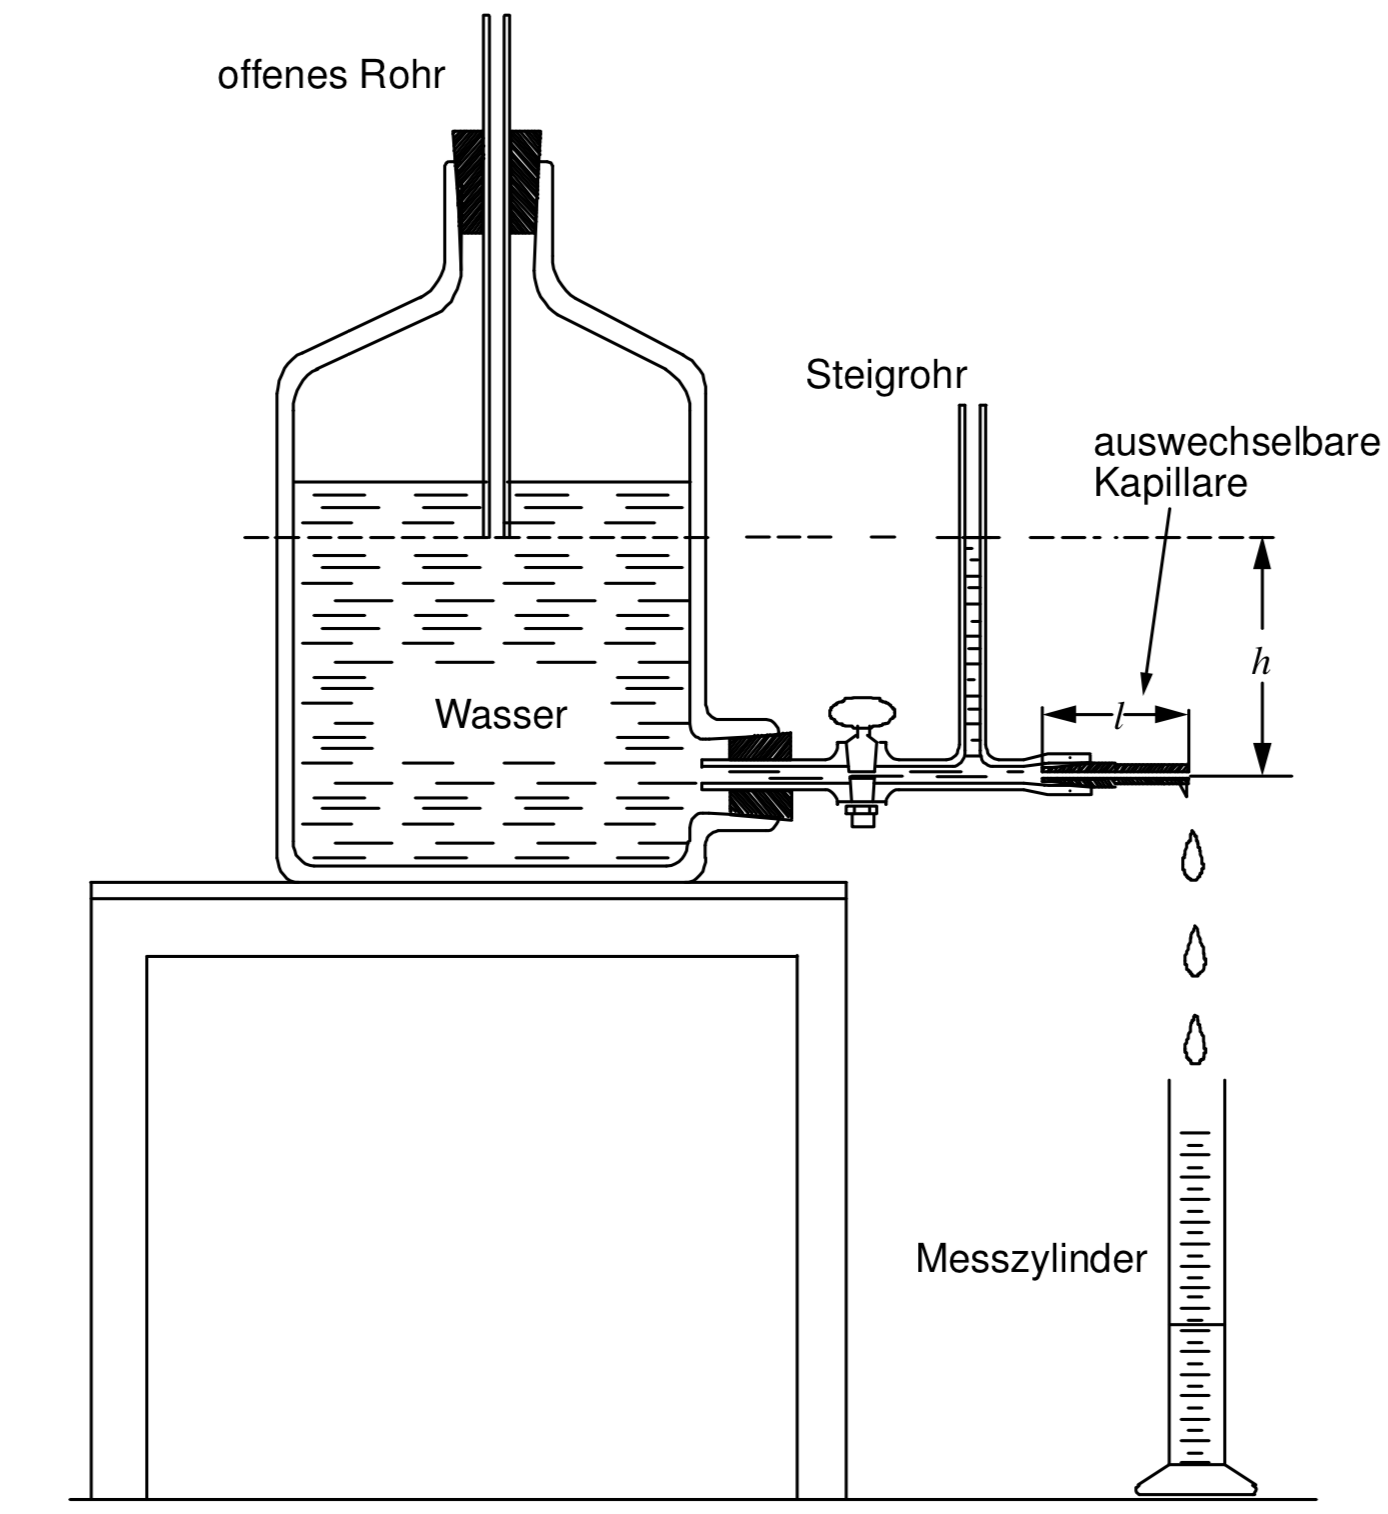
\includegraphics[width=0.5\textwidth]{Meowow}}
   \renewcommand\thefigure{B1}
\caption[Aufbau]{Aufbau \cite{Anleitung}}
\label{Pic:1}
\end{figure}

Für diesen Versuch wurde ein Wasservorratsgefäß, mit einem offenem Rohr, das durch den Deckel geht, verwendet. Dieses Rohr bestimmt die höhe des Wassers im Steigrohr und somit die Druckdifferenz. Es muss genug Wasser vorhanden sein, damit die Wasserhöhe über dem Rohr bleibt. Das Wasservorratsgefäß ist mit einem Hahn an das Steigrohr verbunden. Das Steigrohr hat eine Millimeterskala, womit die Steighöhe des Wassers bestimmt wird. Hier ist zu beachten, dass der Nullpunkt der Skala nicht ganz unten anfängt. Dieser Offset wurde auf das Rohr geschrieben und mit einem Maßband bestätigt. 

Es stehen fünf verschiedene Kapillare zu Verfügung. Diese sind aus Glas und die Angabe deren Länge und Durchmesser wurden in Millimeter dran geklebt. Diese Kapillare können mittels Normschliff mit dem Steigrohr verbunden werden. Zusätzlich wird ein Messzylinder und eine Stoppuhr benötigt, um das Wasservolumen pro Zeit zu messen. Ein Thermometer wird ebenfalls benötigt, um die Temperatur des Wassers zu messen, da die Viskosität stark von der Temperatur abhängig ist.

\pagebreak

\subsection{Durchführung}

Es muss berücksichtigt werden, dass die Druckdifferenz und die Temperatur während des Versuchs konstant bleiben. Die Temperatur wird vor und nach jeder Messreihe überprüft und es wird darauf geachtet, dass die Steighöhe des Wassers vor jeder Messung gleich ist. Eines der verfügbaren Kapillare wird so angebracht, dass das Wasser problemlos durchflie\ss en kann. Ist dies alles eingestellt, so wird der Hahn geöffnet. Ein Becher wird vorerst unter die Öffnung gestellt, bis das Wasser im Steigrohr die erwünschte Höhe angenommen hat. Sobald ein gleichmässiger Wasserstrom fließt, wird der Messzylinder unter die Öffnung gestellt und gleichzeitig die Stoppuhr gestartet. Nach einiger Zeit (bei jeder Messung eine andere) werden gleichzeitig die Stoppuhr gestoppt und der Messzylinder mit dem Becherglas ausgetauscht. Die Werte werden dann aufgeschrieben und sp\"ater in ein Diagramm aufgetragen (siehe Auswertung).

\subsection{Auswertung}

In der Formel $I_V=\frac{V}{t}$ haben sowohl $V$ und $t$ Fehler. Wir verwenden hier also die verallgemeinerte Formel f\"ur Quotienten:
$$
\left\vert\frac{\Delta z}{z}\right\vert=\sqrt{\left(a\frac{\Delta x}{x}\right)^2+\left(b\frac{\Delta y}{y}\right)^2+\ldots}\textrm{ f\"ur }z=x^a\ y^b\ldots
$$
Hier also:
$$
\left\vert\frac{\Delta I_V}{I_V}\right\vert=\sqrt{\left(\frac{\Delta V}{V}\right)^2+\left(-1\frac{\Delta t}{t}\right)^2}
$$
Da $\frac{d^4}{l}$ aus Werten ohne vorhandenem Fehler bestehen, berechnen wir daf\"ur keinen Fehler.

Um unseren Mittelwert zu berechnen, rechnen wir ganz leicht mit 
\begin{equation}
\frac{\sum_{i=1}^n I_{V_i}}{n}\label{mean}
\end{equation}
den Nominalwert, und mit
\begin{equation}
s_x=\sqrt{\frac{1}{n-1}\sum_{i=1}^n(x_i-\overline{x})^2}\label{meanstd}
\end{equation}
die Standardunsichertheit dessen.

Unsere Mittelwerte der $I_V$ f\"ur jede Position werden dann gegen $\frac{d^4}{l}$ aufgetragen, siehe Abbildung (\ref{Abb:1}).

Da wir jedoch klar erkennen k\"onnen, dass $I_{V_4}$ mit der linearen Steigung der anderen Werte nicht \"ubereinstimmt, lassen wir diesen Wert weg und erhalten die Gerade, welche in Abbildung (\ref{Abb:2}) gefunden werden kann.

Um die Steigung der Ausgleichsgeraden zu berechnen, nehmen wir folgende Formel zunutze:
$$
a=\frac{\sum x_i^2\sum y_i-\sum x_i\sum x_iy_i}{n\sum x_i^2-(\sum x_i)^2}
$$

Wir erhalten als Ergebnis daraus f\"ur unser $a$ einen Wert von $(0.041\pm0.009)\,\mathrm{mm}^3$

Um aus unseren Werten $\Delta p$ zu berechnen, verwenden wir
$$
\Delta p=\rho_w hg
$$

Da der einzige Wert mit einem Fehler $h$ ist, rechnen wir einfach mit
$$
\Delta z=\left|\frac{\dif f}{\dif x}\right|\Delta x\textrm{ f\"ur }z=f(x)
$$
unseren Fehler aus.
Mit $\rho_w=1000\,\nicefrac{\mathrm{kg}}{\mathrm{m}^3}$, $g=9.81\,\nicefrac{\mathrm{m}}{\mathrm{s}^2}$ und $h=(135\pm3)\,\mathrm{mm}$ erhalten wir als Wert $\Delta p=(1320\pm30)\,$Pa.

Da wir als Endergebnis $\eta$ wollen, m\"ussen wir erstmal die Gleichung (\ref{hagen}) umstellen und wir erhalten:
$$
\eta=\frac{\pi R^4\Delta p}{8I_V l}.
$$
Hier haben $\Delta p$ und $I_V$ Fehler. Wir wenden also wieder die Gleichung f\"ur Produkte an und erhalten:
$$
\left\vert\frac{\Delta\eta}{\eta}\right\vert=\sqrt{\left(\frac{\Delta\Delta p}{\Delta p}\right)^2+\left(-1\frac{\Delta I_V}{I_V}\right)^2}
$$

Als Ergebnis f\"ur $\eta$ erhalten wir f\"ur unsere vier verwendeten Messreihen:
\begin{itemize}
\item $\eta_1 = (0.8\pm0.17)\,\mathrm{mPa\,s}$
\item $\eta_2 =(1.2\pm0.3)\,\mathrm{mPa\,s}$
\item $\eta_3 =(0.9\pm0.2)\,\mathrm{mPa\,s}$
\item $\eta_4 =(0.9\pm0.2)\,\mathrm{mPa\,s}$
\end{itemize}


Nutzen wir die Formeln (\ref{mean}) und (\ref{meanstd}) um unseren Mittelwert zu bestimmen, so erhalten wir als Standardunsicherheit
\[
\overline{\eta} = (0.8\pm0.18)\,\mathrm{mPa\,s}
\]

Als n\"achstes betrachten wir den durchschnittlichen Fehler der Messungen und die Streuung:

Wir erhalten als durchschnittlichen Fehler $0.0065\,$mL und als Streuung $0.0604\,$mL. Diese Werte implizieren gute Messwerte, da der Fehler wesentlich geringer als die Streuung ist.

Anhand der Fehlerbalken ist zu erkennen, dass der Fehler mit zunehmenden $\frac{d^4}{l}$ steigt. Da die Formel f\"ur $I_V$ zu  $\frac{1}{l}$ und $\left(\frac{d}{2}\right)^2$ proportional ist, aber diese Werte keine statistischen Fehler haben, ist klar, dass dies aufgrund von systematischer Fehler der Fall sein muss.
\section{Diskussion}

Mit einer Temperatur $(21\pm 1)\celsius$ ist der Literaturwert $\eta_L = 0.98\pm 0.02$\,Pa\,s \cite{Litval}. Dieser Wert ist mit unserem Wert kompatibel, denn die Abweichung ist $t \approx 1$ welches mit:
$$t = \frac{|\overline{\eta}-\eta_L|}{\sqrt{\overline{u}^2 + u_L^2}}$$
berechnet wurde. Somit gilt $t<2$, dies deutet darauf hin, dass die Auswirkung der Fehler gering ist. Außer den Messunsicherheiten von Volumen, Steighöhe und Zeit, gibt es zusätzliche vermeidbare Fehlerquellen. Erstens ist die Steighohe des Wassers nicht komplett konstant da es durch das Einströmen von Luft $\approx 3$\,mm schwankt. Das synchrone Starten und Stoppen von der Stoppuhr und hinunter schieben beziehungsweise wegziehen des Messzylinders ist von der Reaktionszeit abhängig, dieser Fehler kann verringert werden durch längeres Messen. Der Rest Wasser in dem Zylinder von vorherigen Messungen ist auch ein leicht vermeidbarer Fehler, aber dieser ist kleiner als die Unsicherheit des Messzylinders. Also für exaktere Werte müssen erstmals genauere Instrumente verwendet werden. Die geringe Auswirkung der Fehler deutet darauf hin, dass das Wasser rein war und es keine Verstopfung, oder undichte stellen gab. 

\begin{thebibliography}{9}
%\bibitem{Uncertainties}''Correlations between variables are automatically handled, which sets this module apart from many existing error propagation codes.'' - \url{https://pythonhosted.org/uncertainties/}
\bibitem{Anleitung} Physikalisches Institut der Albert-Ludwigs-Universität Freiburg (Hrsg.) (08/2018): Versuchsanleitungen zum Physiklabor für Anfänger*innen, Teil 1, Ferienpraktikum im Sommersemester 2018.
\bibitem{Litval} Viscosity of Water:  \url{https://wiki.anton-paar.com/en/water/}\\ Abrufdatum: \today
\end{thebibliography}

\pagebreak

\section{Anhang: Tabellen und Diagramme}

\begin{figure}[h]
\centering
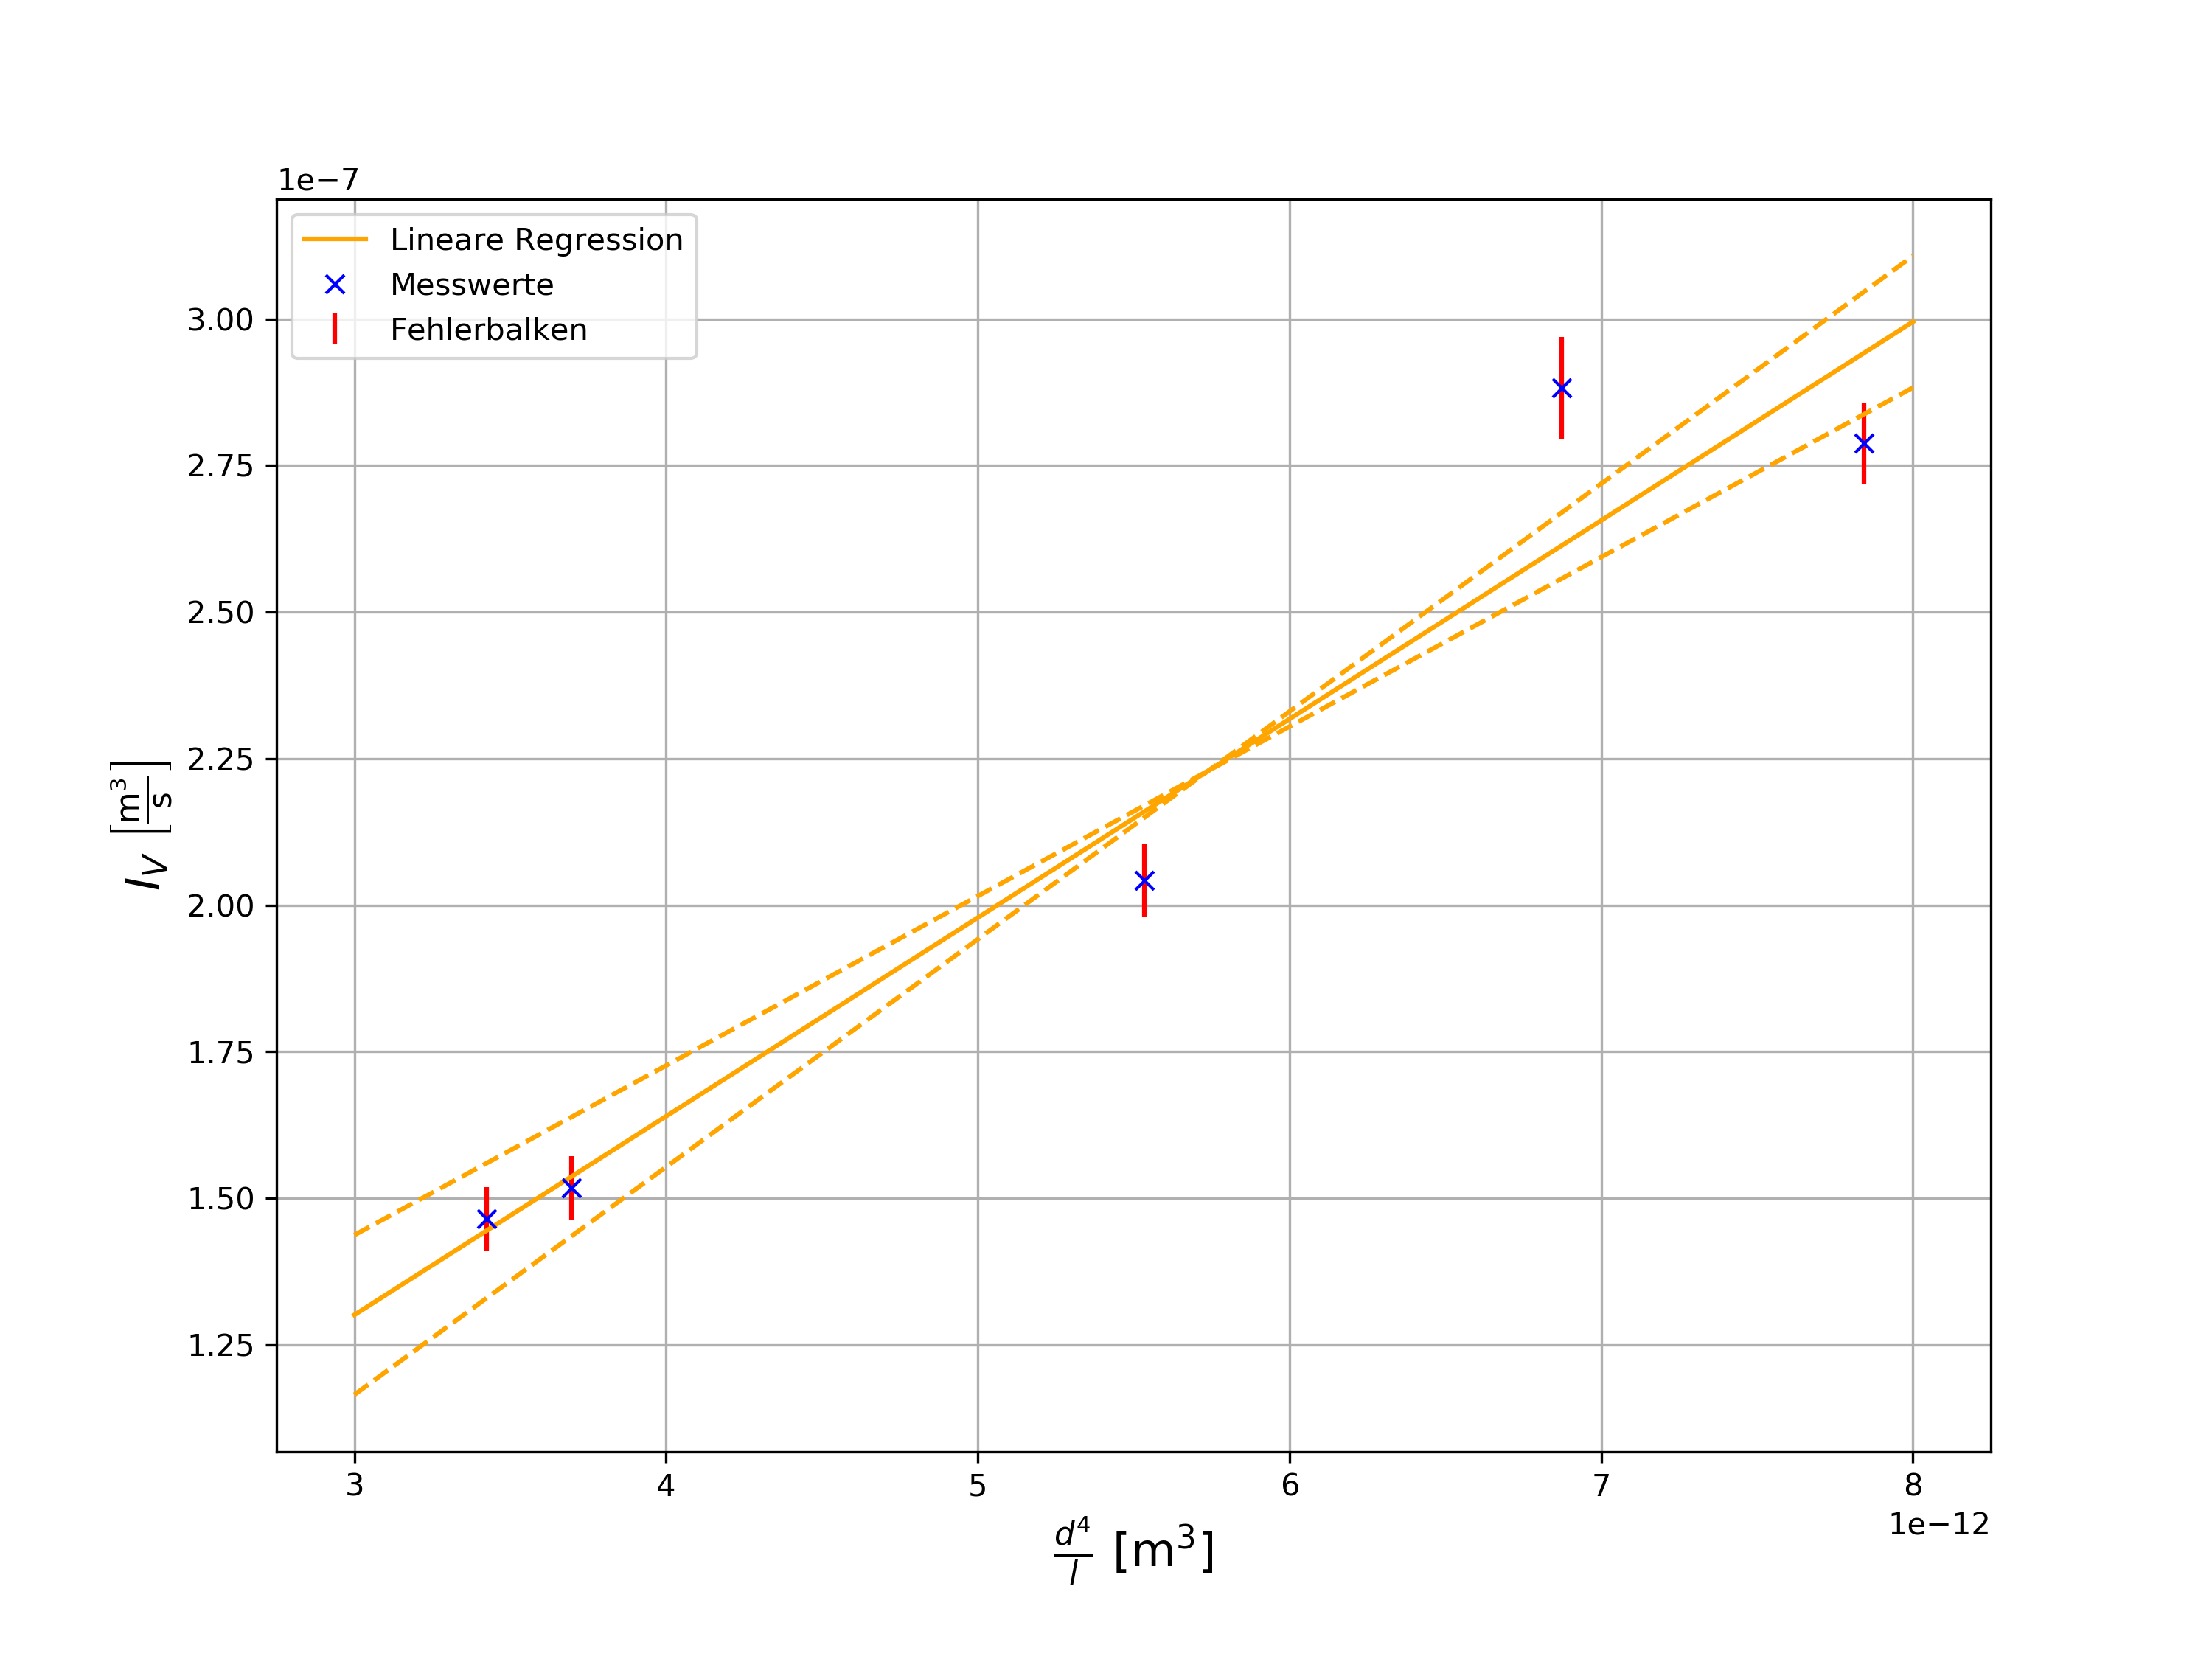
\includegraphics[width=0.7\textwidth]{graph_with_5}
\renewcommand\thefigure{B2}\vspace{-22pt}
\caption[Graph mit allen Messergebnissen]{Graph mit allen Messergebnissen}
\label{Abb:1}
\end{figure}

\begin{figure}[h]
\centering
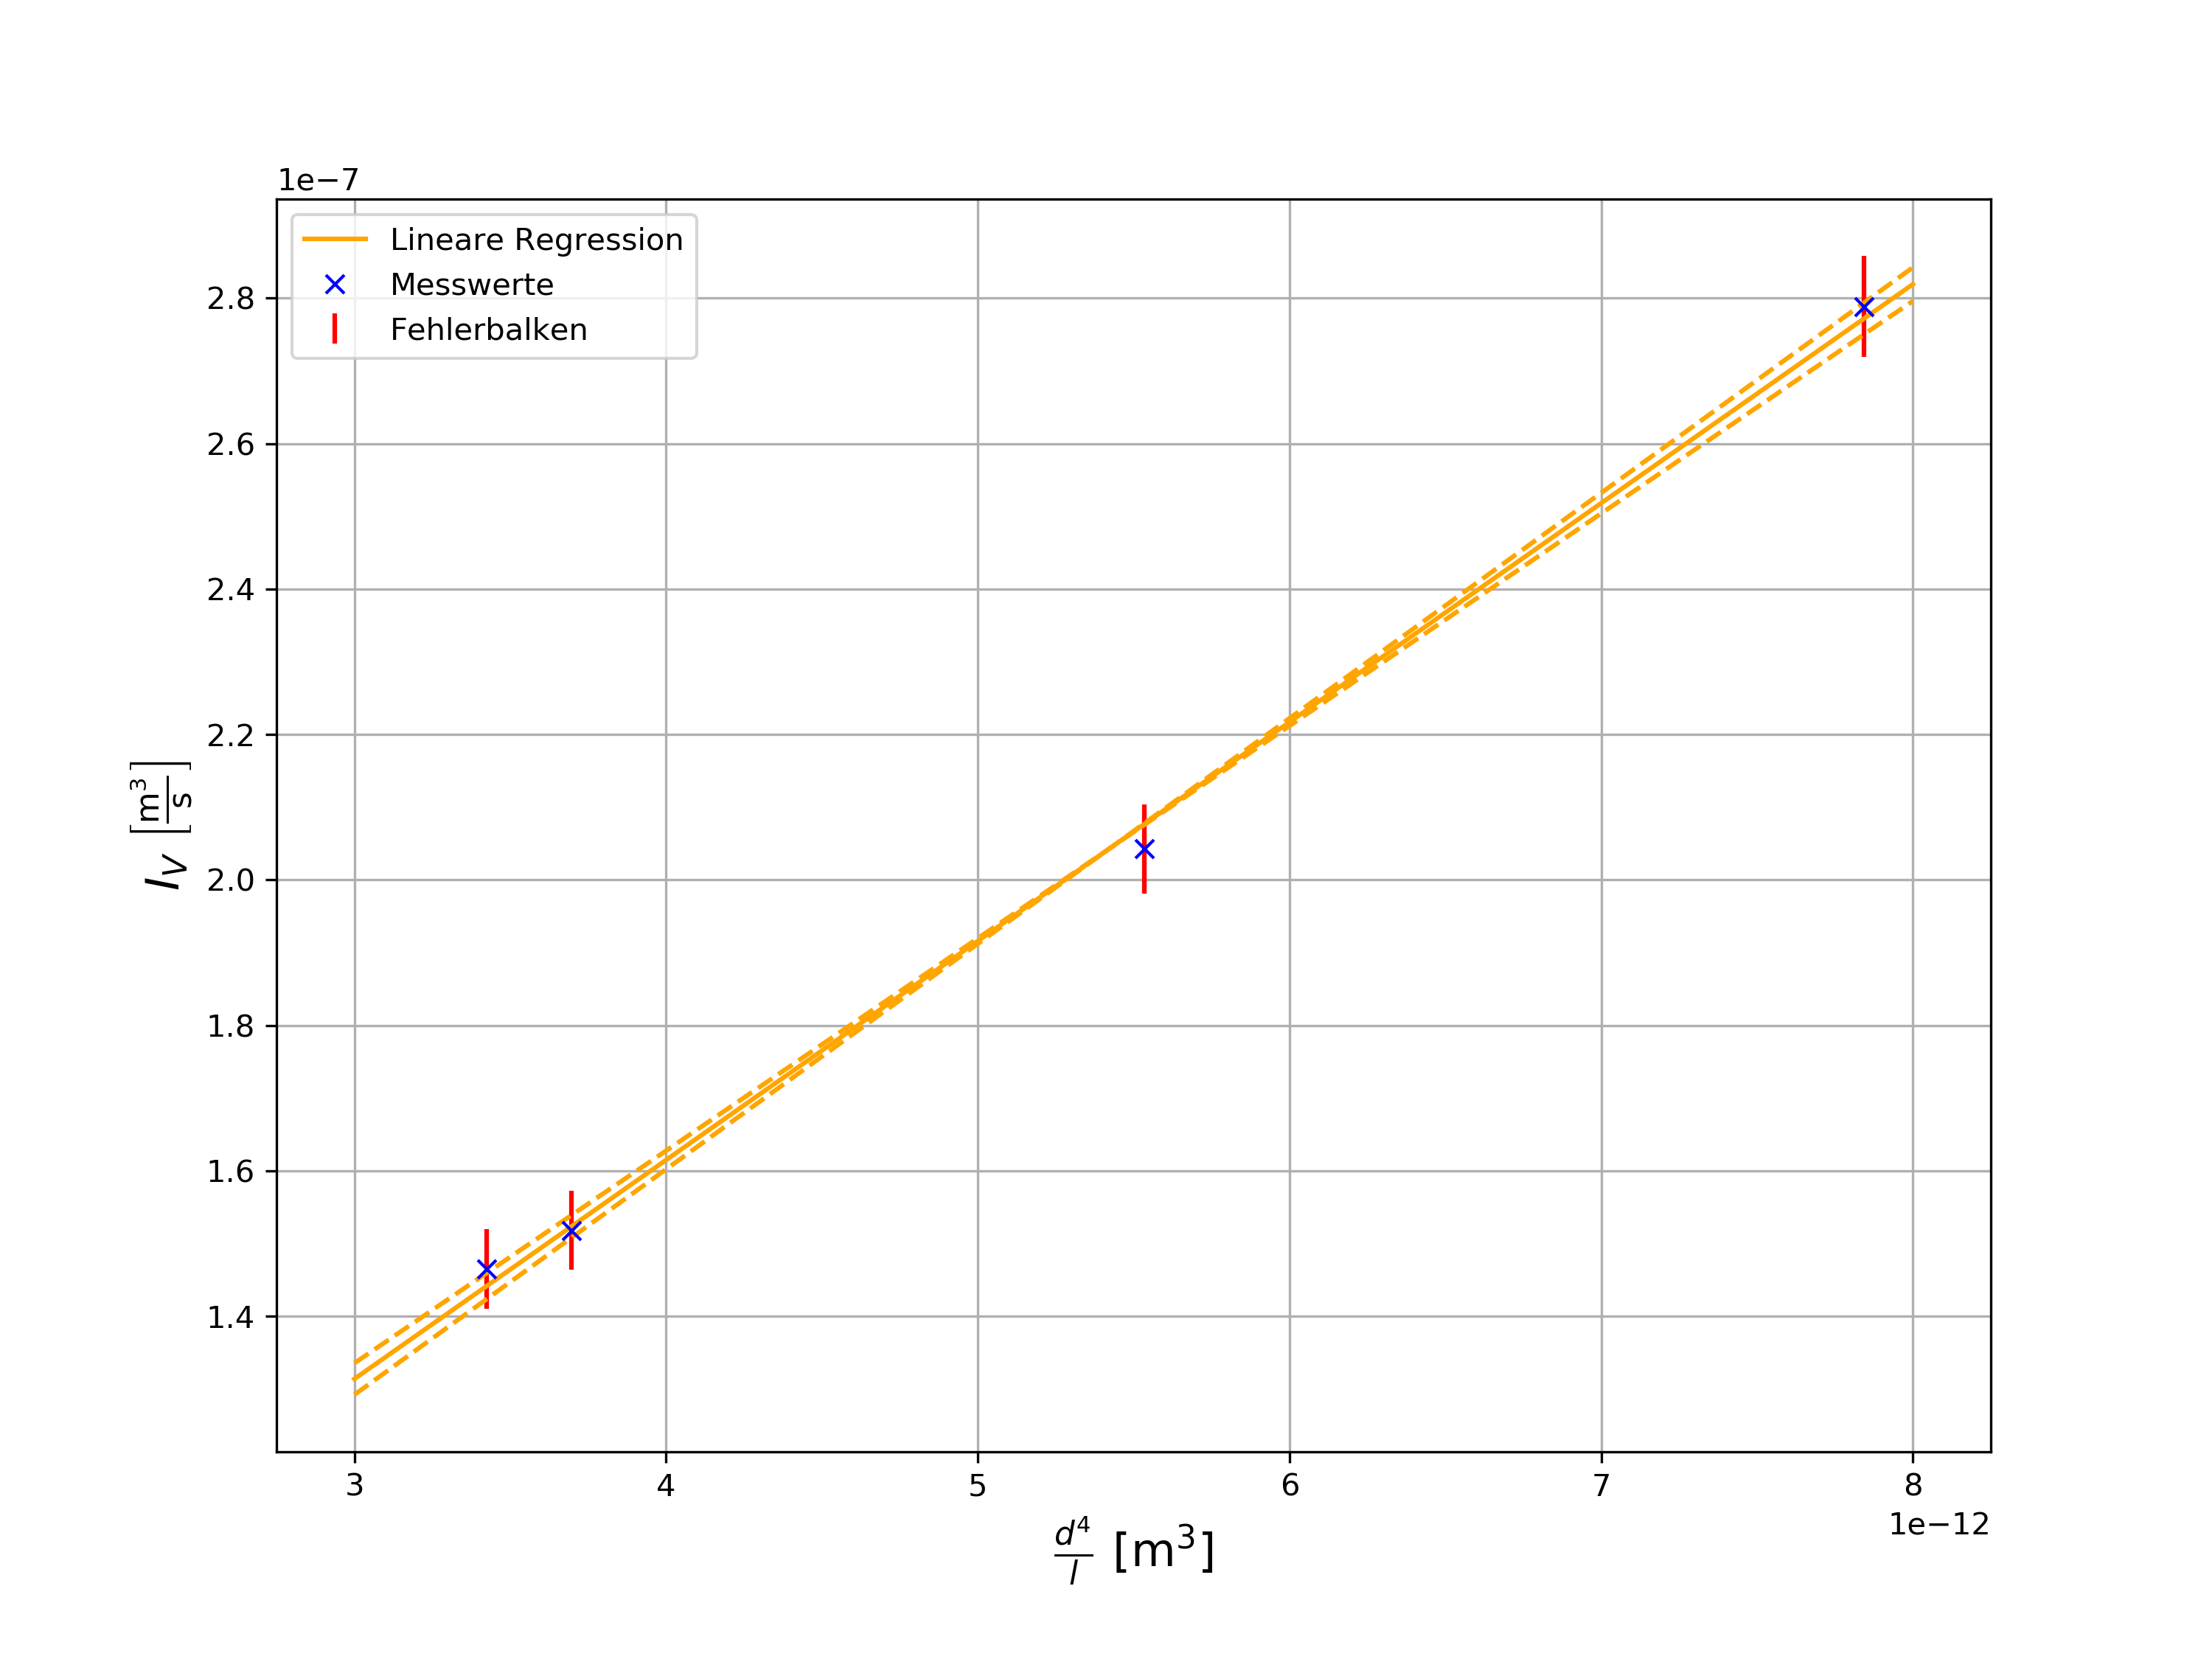
\includegraphics[width=0.7\textwidth]{graph_without_5}
\renewcommand\thefigure{B3}\vspace{-22pt}
\caption[Graph ohne sinnloses Messergebnis]{Graph ohne sinnloses Messergebnis}
\label{Abb:2}
\end{figure}

\end{document}